\documentclass{article}\usepackage[]{graphicx}\usepackage[]{color}
%% maxwidth is the original width if it is less than linewidth
%% otherwise use linewidth (to make sure the graphics do not exceed the margin)
\makeatletter
\def\maxwidth{ %
  \ifdim\Gin@nat@width>\linewidth
    \linewidth
  \else
    \Gin@nat@width
  \fi
}
\makeatother

\definecolor{fgcolor}{rgb}{0.345, 0.345, 0.345}
\newcommand{\hlnum}[1]{\textcolor[rgb]{0.686,0.059,0.569}{#1}}%
\newcommand{\hlstr}[1]{\textcolor[rgb]{0.192,0.494,0.8}{#1}}%
\newcommand{\hlcom}[1]{\textcolor[rgb]{0.678,0.584,0.686}{\textit{#1}}}%
\newcommand{\hlopt}[1]{\textcolor[rgb]{0,0,0}{#1}}%
\newcommand{\hlstd}[1]{\textcolor[rgb]{0.345,0.345,0.345}{#1}}%
\newcommand{\hlkwa}[1]{\textcolor[rgb]{0.161,0.373,0.58}{\textbf{#1}}}%
\newcommand{\hlkwb}[1]{\textcolor[rgb]{0.69,0.353,0.396}{#1}}%
\newcommand{\hlkwc}[1]{\textcolor[rgb]{0.333,0.667,0.333}{#1}}%
\newcommand{\hlkwd}[1]{\textcolor[rgb]{0.737,0.353,0.396}{\textbf{#1}}}%
\let\hlipl\hlkwb

\usepackage{framed}
\makeatletter
\newenvironment{kframe}{%
 \def\at@end@of@kframe{}%
 \ifinner\ifhmode%
  \def\at@end@of@kframe{\end{minipage}}%
  \begin{minipage}{\columnwidth}%
 \fi\fi%
 \def\FrameCommand##1{\hskip\@totalleftmargin \hskip-\fboxsep
 \colorbox{shadecolor}{##1}\hskip-\fboxsep
     % There is no \\@totalrightmargin, so:
     \hskip-\linewidth \hskip-\@totalleftmargin \hskip\columnwidth}%
 \MakeFramed {\advance\hsize-\width
   \@totalleftmargin\z@ \linewidth\hsize
   \@setminipage}}%
 {\par\unskip\endMakeFramed%
 \at@end@of@kframe}
\makeatother

\definecolor{shadecolor}{rgb}{.97, .97, .97}
\definecolor{messagecolor}{rgb}{0, 0, 0}
\definecolor{warningcolor}{rgb}{1, 0, 1}
\definecolor{errorcolor}{rgb}{1, 0, 0}
\newenvironment{knitrout}{}{} % an empty environment to be redefined in TeX

\usepackage{alltt}

%\VignetteEngine{knitr::knitr}
%\VignetteIndexEntry{Spatio-temporal modelling with IDE}

\usepackage{amssymb,amsmath,amstext}
\usepackage{algorithm}
\usepackage{algpseudocode}
\usepackage{color}
\usepackage{dcolumn}
\usepackage{dsfont}
\usepackage{epsfig}
\usepackage[T1]{fontenc}
\usepackage[]{graphicx}
\usepackage{ifthen}
\usepackage{longtable}
\usepackage{makeidx}
\usepackage{natbib}
\usepackage{setspace}
\usepackage{multirow}
\usepackage{tabularx}
\usepackage{threeparttable}
\usepackage{times}
\usepackage{titlesec}
\usepackage{url}
\usepackage{verbatim}

\newcommand{\mbf}[1]{\mathbf{#1}}
\newcommand{\mbv}[1]{\mbox{\boldmath$#1$\unboldmath}}
\newcommand{\bfu}{{ \bf u}}
\def\ba{\mathbf{a}}
\def\bb{\mathbf{b}}
\def\bc{\mathbf{c}}
\def\bd{\mathbf{d}}
\def\be{\mathbf{e}}
\def\bg{\mathbf{g}}
\def\bh{\mathbf{h}}
\def\bk{\mathbf{k}}
\def\bm{\mathbf{m}}
\def\br{\mathbf{r}}
\def\bs{\mathbf{s}}
\def\bu{\mathbf{u}}
\def\bv{\mathbf{v}}
\def\bw{\mathbf{w}}
\def\bx{\mathbf{x}}
\def\by{\mathbf{y}}
\def\bz{\mathbf{z}}
\def\bA{\mathbf{A}}
\def\bB{\mathbf{B}}
\def\bC{\mathbf{C}}
\def\bD{\mathbf{D}}
\def\bE{\mathbf{E}}
\def\bF{\mathbf{F}}
\def\bG{\mathbf{G}}
\def\bH{\mathbf{H}}
\def\bI{\mathbf{I}}
\def\bJ{\mathbf{J}}
\def\bK{\mathbf{K}}
\def\bL{\mathbf{L}}
\def\bM{\mathbf{M}}
\def\bP{\mathbf{P}}
\def\bQ{\mathbf{Q}}
\def\bR{\mathbf{R}}
\def\bS{\mathbf{S}}
\def\bT{\mathbf{T}}
\def\bU{\mathbf{U}}
\def\bV{\mathbf{V}}
\def\bW{\mathbf{W}}
\def\bX{\mathbf{X}}
\def\bY{\mathbf{Y}}
\def\bZ{\mathbf{Z}}
\def\bfzero{\mathbf{0}}
\def\bfone{\mathbf{1}}

\newcommand{\intd}{\textrm{d}}
\newcommand{\bfomega}{\mbox{\boldmath $\omega$}}
\newcommand{\bfalpha}{\mbox{\boldmath $\alpha$}}
\newcommand{\bfbeta}{\mbox{\boldmath $\beta$}}
\newcommand{\bfxi}{\mbox{\boldmath $\xi$}}
\newcommand{\bfeta}{\mbox{\boldmath $\eta$}}
\newcommand{\bftau}{\mbox{\boldmath $\tau$}}
\newcommand{\bfdelta}{\mbox{\boldmath $\delta$}}
\newcommand{\bftheta}{\mbox{\boldmath $\theta$}}
\newcommand{\bfTheta}{\mbox{\boldmath $\Theta$}}
\newcommand{\bfell}{\mbox{\boldmath $\ell$}}
\newcommand{\bfepsilon}{\mbox{\boldmath $\varepsilon$}}
\newcommand{\bfPhi}{\mbox{\boldmath $\Phi$}}
\newcommand{\bfPsi}{\mbox{\boldmath $\Psi$}}
\newcommand{\bfpsi}{\mbox{\boldmath $\psi$}}
\newcommand{\bfphi}{\mbox{\boldmath $\phi$}}
\newcommand{\bfmu}{\mbox{\boldmath $\mu$}}
\newcommand{\bfsigma}{\mbox{\boldmath $\sigma$}}
\newcommand{\bfnu}{\mbox{\boldmath $\nu$}}
\newcommand{\bfgamma}{\mbox{\boldmath $\gamma$}}
\newcommand{\bflambda}{\mbox{\boldmath $\lambda$}}
\newcommand{\bfLambda}{\mbox{\boldmath $\Lambda$}}
\newcommand{\bfSigma}{\mbox{\boldmath $\Sigma$}}
\newcommand{\bfPi}{\mbox{\boldmath $\Pi$}}
\newcommand{\var}{\textrm{var}}
\newcommand{\cov}{\textrm{cov}}
\newcommand{\bdiag}{\textrm{bdiag}}
\newcommand{\corr}{\textrm{corr}}
\newcommand{\pr}{\textrm{Pr}}
\newcommand{\fn}[1]{\texttt{\hlkwd{#1}}}
\newcommand{\num}[1]{\texttt{\hlnum{#1}}}
\newcommand{\strn}[1]{\texttt{\hlstr{#1}}}
\newcommand{\args}[1]{\texttt{\hlkwc{#1}}}
\newcommand{\R}{\texttt{R}}
\newcommand{\cc}[1]{\texttt{#1}}
\def\deg{$^{\circ}$ }
\newcommand{\rf}{\vskip .1in\par\sloppy\hangindent=1pc\hangafter=1
                 \noindent}

\newcommand{\indexprint}[1]{#1\index{#1}}

\DeclareMathOperator{\diag}{diag}
\DeclareMathOperator{\Gau}{Gau}
\DeclareMathOperator{\trace}{trace}
\DeclareMathOperator{\tr}{tr}

\usepackage[margin=1in,includefoot,includehead]{geometry}


\bibliographystyle{plainnat}

\title{Spatio-temporal IDE modelling: The \tt{R} package}
\author{Andrew Zammit-Mangion}
%\author[1]{Noel Cressie}
%\affiliation{National Institute for Applied Statistics Research Australia~(NIASRA), School of Mathematics and Applied Statistics, University of Wollongong, New South Wales 2522, Australia}
\IfFileExists{upquote.sty}{\usepackage{upquote}}{}
\begin{document}



%\SweaveOpts{concordance=TRUE}

\maketitle


In this vignette we use the package {\bf IDE} to fit spatio-temporal IDE models, as well as predict and forecast from spatio-temporal data. We will explore two cases using simulated data where the true model is known. For this vignette, we need the following packages:

\begin{knitrout}
\definecolor{shadecolor}{rgb}{0.969, 0.969, 0.969}\color{fgcolor}\begin{kframe}
\begin{alltt}
\hlkwd{library}\hlstd{(}\hlstr{"dplyr"}\hlstd{)}
\hlkwd{library}\hlstd{(}\hlstr{"FRK"}\hlstd{)}
\hlkwd{library}\hlstd{(}\hlstr{"ggplot2"}\hlstd{)}
\hlkwd{library}\hlstd{(}\hlstr{"sp"}\hlstd{)}
\hlkwd{library}\hlstd{(}\hlstr{"spacetime"}\hlstd{)}
\end{alltt}
\end{kframe}
\end{knitrout}




The first-order spatio-temporal IDE process model used in the package {\bf IDE} is given by
\begin{equation}
Y_t(\bs) = \int_{D_s} m(\bs,\bx;\bftheta_p) Y_{t-1}(\bx) \; \intd \bx  + \eta_t(\bs); \;\;\; \bs,\bx \in D_s,
\label{eq:linearIDE}
\end{equation}
for $t=1,2,\ldots$, where $m(\bs,\bx;\bftheta_p)$ is a {\it transition kernel}, depending on parameters $\bftheta_p$ that specify ``redistribution weights'' for the process at the previous time over the spatial domain, $D_s$, and $\eta_t(\bs)$ is a time-varying (but statistically independent in time) continuous mean-zero Gaussian spatial process.   Note that it is assumed here that the parameter vector $\bftheta_p$ does not vary with time, as one often does, but it could in general.  So, the process at location $\bs$ and time $t$ is given by the weighted average (integral) of the process throughout the domain at the past time, where the weights are given by the transition kernel, $m(\cdot)$.  The ``adjustment,'' given by $\eta_t(\bs)$, is assumed to be Gaussian and accounts for spatial dependencies in $Y_t(\cdot)$ that are not captured by this weighted average. Another way to think about $\eta_t(\cdot)$ is that it adds smaller-scale dependence that is removed in the inherent smoothing that occurs when $\{Y_{t-1}(\cdot)\}$ is averaged over space, in order to give $Y_t(\cdot)$ a realistic spatial dependence structure. In general, $\int_{D_s} m(\bs,\bx;\bftheta_p) \intd \bx < 1$ for the process to be stable (non-explosive) in time.

The redistribution kernel $m(\bs,\bx;\bftheta_p)$ used by the package {\bf IDE} is given by

\begin{equation}
%m(s,x;\bftheta_p) = \frac{1}{\theta_{p,2} \sqrt{2 \pi}} \exp\left(-\frac{1}{2 \; \theta_{p,2}}(x - \theta_{p,1} - s)^2 \right) ,
m(\bs,\bx;\bftheta_p) = {\theta_{p,1}(\bs)} \exp\left(-\frac{1}{\theta_{p,2}(\bs)}\left[(x_1 - \theta_{p,3}(\bs) - s_1)^2 + (x_2 - \theta_{p,4}(\bs) - s_2)^2 \right] \right),
\label{eq:Gausskern}
\end{equation}

\noindent where the spatially-varying kernel amplitude is given by $\theta_{p,1}(\bs)$ and controls the temporal stationarity, the spatially-varying length-scale (variance) parameter $\theta_{p,2}(\bs)$ corresponds to a kernel scale (aperture) parameter (i.e., the kernel width increases as $\theta_{p,2}$ increases), and the mean (shift) parameters $\theta_{p,3}(\bs)$ and $\theta_{p,4}(\bs)$ correspond to a spatially-varying shift of the kernel relative to location $\bs$. Spatially-invariant kernels (i.e., where the elements of $\bftheta_p$ are not functions of space) are also allowed.

\subsection*{Simulation example with a spatially-invariant kernel}

The package {\bf IDE} contains a function \fn{simIDE} that simulates the behaviour of a typical dynamic system governed by linear transport. The function takes just three arguments, the number of time points to simulate, the number of (spatially fixed) observations to use, and a flag indicating whether to use a spatially-invariant kernel or not.

\begin{knitrout}
\definecolor{shadecolor}{rgb}{0.969, 0.969, 0.969}\color{fgcolor}\begin{kframe}
\begin{alltt}
\hlstd{SIM1} \hlkwb{<-} \hlkwd{simIDE}\hlstd{(}\hlkwc{T} \hlstd{=} \hlnum{10}\hlstd{,} \hlkwc{nobs} \hlstd{=} \hlnum{100}\hlstd{,} \hlkwc{k_spat_invariant} \hlstd{=} \hlnum{1}\hlstd{)}
\end{alltt}
\end{kframe}
\end{knitrout}

\noindent The returned list \cc{SIM1} contains the simulated process in the data frame \cc{s\_df}, the observed data in the data frame \cc{z\_df}, and also as an \cc{STIDF} object \cc{z\_STIDF}. It also contains two {\bf ggplot2} plots, \cc{g\_truth} and \cc{g\_obs} which can be readily plotted as follows.

\begin{knitrout}
\definecolor{shadecolor}{rgb}{0.969, 0.969, 0.969}\color{fgcolor}\begin{kframe}
\begin{alltt}
\hlkwd{print}\hlstd{(SIM1}\hlopt{$}\hlstd{g_truth)}
\hlkwd{print}\hlstd{(SIM1}\hlopt{$}\hlstd{g_obs)}
\end{alltt}
\end{kframe}
\end{knitrout}

\noindent While the transport action is clearly noticeable in the process evolution, there is also a clear spatial trend. Covariates are included through the use of a standard \cc{R} formula when calling the function \fn{IDE}. Additional arguments to \fn{IDE} include the dataset, which needs to be of class \cc{STIDF}, the temporal discretization to use (we will use 1 day) of class \cc{difftime}, and the gridsize on which the integrations (as well as predictions) will be carried out. Other arguments include user-specified basis functions for the process and the transition kernel, which for now we will not specify. By default, the IDE model will decompose the process using two resolutions of bisquare basis functions, and assume a spatially-invariant Gaussian transition kernel.

\begin{knitrout}
\definecolor{shadecolor}{rgb}{0.969, 0.969, 0.969}\color{fgcolor}\begin{kframe}
\begin{alltt}
\hlstd{IDEmodel} \hlkwb{<-} \hlkwd{IDE}\hlstd{(}\hlkwc{f} \hlstd{= z} \hlopt{~} \hlstd{s1} \hlopt{+} \hlstd{s2,}
                \hlkwc{data} \hlstd{= SIM1}\hlopt{$}\hlstd{z_STIDF,}
                \hlkwc{dt} \hlstd{=} \hlkwd{as.difftime}\hlstd{(}\hlnum{1}\hlstd{,} \hlkwc{units} \hlstd{=} \hlstr{"days"}\hlstd{),}
                \hlkwc{grid_size} \hlstd{=} \hlnum{41}\hlstd{)}
\end{alltt}
\end{kframe}
\end{knitrout}

The returned object \cc{IDEmodel} is of class \cc{IDE} and contains initial parameter estimates, as well as predictions for $\bfalpha_t, t = 1,\dots,T$ at these initial parameter estimates. The parameters in this case are the measurement-error variance, the variance of the random disturbance $\eta_t(\bs)$ (whose covariance structure is fixed), the kernel parameters, and the regression coefficients $\bfbeta$.

Fitting the IDE is a computationally intensive procedure. The default method currently implemented uses a differential evolution optimization algorithm from the package {\bf DEoptim}, which is a global optimization algorithm that can be easily parallelized. Fitting takes only a few minutes on a 60-core machine but can take an hour or two on a standard desktop. Fitting can be done by running

\begin{knitrout}
\definecolor{shadecolor}{rgb}{0.969, 0.969, 0.969}\color{fgcolor}\begin{kframe}
\begin{alltt}
\hlstd{fit_results_sim1} \hlkwb{<-} \hlkwd{fit.IDE}\hlstd{(IDEmodel,}
                           \hlkwc{parallelType} \hlstd{=} \hlnum{1}\hlstd{)}
\end{alltt}
\end{kframe}
\end{knitrout}

\noindent where \args{parallelType}\cc{ = }\num{1} ensures that all available cores on the machine are used for fitting. Alternatively, the results can be loaded from cache as follows





\begin{knitrout}
\definecolor{shadecolor}{rgb}{0.969, 0.969, 0.969}\color{fgcolor}\begin{kframe}
\begin{alltt}
\hlkwd{data}\hlstd{(}\hlstr{"IDE_Sim1_results"}\hlstd{)}
\end{alltt}
\end{kframe}
\end{knitrout}

The list \cc{fit\_results\_sim1} contains two fields: \cc{optim\_results} that contains the output of the optimization algorithm, and \cc{IDEmodel} that contains the fitted IDE model. The fitted kernel can be visualized by using the function \fn{show\_kernel}.

\begin{knitrout}
\definecolor{shadecolor}{rgb}{0.969, 0.969, 0.969}\color{fgcolor}\begin{kframe}
\begin{alltt}
\hlkwd{show_kernel}\hlstd{(fit_results_sim1}\hlopt{$}\hlstd{IDEmodel)}
\end{alltt}
\end{kframe}
\end{knitrout}

\noindent Note how the fitted kernel is shifted to the left and upwards, correctly representing the south-easterly transport evident in the data. The estimated kernel parameters $\bftheta_p$ are

\begin{knitrout}
\definecolor{shadecolor}{rgb}{0.969, 0.969, 0.969}\color{fgcolor}\begin{kframe}
\begin{alltt}
\hlstd{fit_results_sim1}\hlopt{$}\hlstd{IDEmodel}\hlopt{$}\hlkwd{get}\hlstd{(}\hlstr{"k"}\hlstd{)} \hlopt \hlkwd{unlist}\hlstd{()}
\end{alltt}
\end{kframe}
\end{knitrout}
\noindent which can be compared to the true values \cc{c(}\num{150}, \num{0.002}, \num{-0.1}, \num{0.1}\cc{)}. The estimated amplitude is lower and the aperture is larger than those values used to simulate the true field, but the shift parameters are remarkably similar. The estimated regression coefficients are

\begin{knitrout}
\definecolor{shadecolor}{rgb}{0.969, 0.969, 0.969}\color{fgcolor}\begin{kframe}
\begin{alltt}
\hlstd{fit_results_sim1}\hlopt{$}\hlstd{IDEmodel}\hlopt{$}\hlkwd{get}\hlstd{(}\hlstr{"betahat"}\hlstd{)}
\end{alltt}
\end{kframe}
\end{knitrout}

\noindent which also compare well to the true values \cc{c(}\num{0.2}, \num{0.2}, \num{0.2}\c{)}. Also of interest are the modulus of the eigenvalues of the evolution matrix $\bM$. These can be extracted as follows.

\begin{knitrout}
\definecolor{shadecolor}{rgb}{0.969, 0.969, 0.969}\color{fgcolor}\begin{kframe}
\begin{alltt}
\hlstd{abs_ev} \hlkwb{<-} \hlkwd{eigen}\hlstd{(fit_results_sim1}\hlopt{$}\hlstd{IDEmodel}\hlopt{$}\hlkwd{get}\hlstd{(}\hlstr{"M"}\hlstd{))}\hlopt{$}\hlstd{values} \hlopt \hlkwd{abs}\hlstd{()}
\hlkwd{summary}\hlstd{(abs_ev)}
\end{alltt}
\end{kframe}
\end{knitrout}

\noindent Since the largest of these is less than 1, the IDE process exhibits stable behavior.

For prediction, one may either specify a prediction grid, or use the default one used for approximating the integrations set up by \fn{IDE}. The latter is usually sufficient so we use this without exception for the examples we consider. %In the former, one should specify an \cc{STFDF}, for example as follows.
When a prediction grid is not supplied, the function \fn{predict} returns a data frame with predictions spanning the data temporal horizon (forecasts and hindcasts are explored later).

\begin{knitrout}
\definecolor{shadecolor}{rgb}{0.969, 0.969, 0.969}\color{fgcolor}\begin{kframe}
\begin{alltt}
\hlstd{ST_grid_df} \hlkwb{<-} \hlkwd{predict}\hlstd{(fit_results_sim1}\hlopt{$}\hlstd{IDEmodel)}
\end{alltt}
\end{kframe}
\end{knitrout}

The prediction and prediction standard error can now be plotted using standard {\bf ggplot2} commands as follows.

\begin{knitrout}
\definecolor{shadecolor}{rgb}{0.969, 0.969, 0.969}\color{fgcolor}\begin{kframe}
\begin{alltt}
\hlstd{gpred} \hlkwb{<-} \hlkwd{ggplot}\hlstd{(ST_grid_df)} \hlopt{+}             \hlcom{# Plot the predictions}
  \hlkwd{geom_tile}\hlstd{(}\hlkwd{aes}\hlstd{(s1, s2,} \hlkwc{fill}\hlstd{=Ypred))} \hlopt{+}
  \hlkwd{facet_wrap}\hlstd{(}\hlopt{~}\hlstd{t)} \hlopt{+}
  \hlkwd{scale_fill_distiller}\hlstd{(}\hlkwc{palette}\hlstd{=}\hlstr{"Spectral"}\hlstd{,} \hlkwc{limits} \hlstd{=} \hlkwd{c}\hlstd{(}\hlopt{-}\hlnum{0.1}\hlstd{,}\hlnum{1.4}\hlstd{))} \hlopt{+}
  \hlkwd{coord_fixed}\hlstd{(}\hlkwc{xlim}\hlstd{=}\hlkwd{c}\hlstd{(}\hlnum{0}\hlstd{,} \hlnum{1}\hlstd{),} \hlkwc{ylim} \hlstd{=} \hlkwd{c}\hlstd{(}\hlnum{0}\hlstd{,} \hlnum{1}\hlstd{))}

\hlstd{gpredse} \hlkwb{<-} \hlkwd{ggplot}\hlstd{(ST_grid_df)} \hlopt{+}           \hlcom{# Plot the prediction s.es}
  \hlkwd{geom_tile}\hlstd{(}\hlkwd{aes}\hlstd{(s1, s2,} \hlkwc{fill}\hlstd{=Ypredse))} \hlopt{+}
  \hlkwd{facet_wrap}\hlstd{(}\hlopt{~}\hlstd{t)} \hlopt{+}
  \hlkwd{scale_fill_distiller}\hlstd{(}\hlkwc{palette}\hlstd{=}\hlstr{"Spectral"}\hlstd{)} \hlopt{+}
  \hlkwd{coord_fixed}\hlstd{(}\hlkwc{xlim}\hlstd{=}\hlkwd{c}\hlstd{(}\hlnum{0}\hlstd{,} \hlnum{1}\hlstd{),} \hlkwc{ylim} \hlstd{=} \hlkwd{c}\hlstd{(}\hlnum{0}\hlstd{,} \hlnum{1}\hlstd{))}
\end{alltt}
\end{kframe}
\end{knitrout}

\noindent In Figure~\ref{fig:IDEsimresults}, we show the observations, the true process, the predictions, and the prediction standard errors from the fitted model. Note how prediction standard errors are high in regions of sparse observations, as expected.



\begin{figure}[t!]
\begin{center}
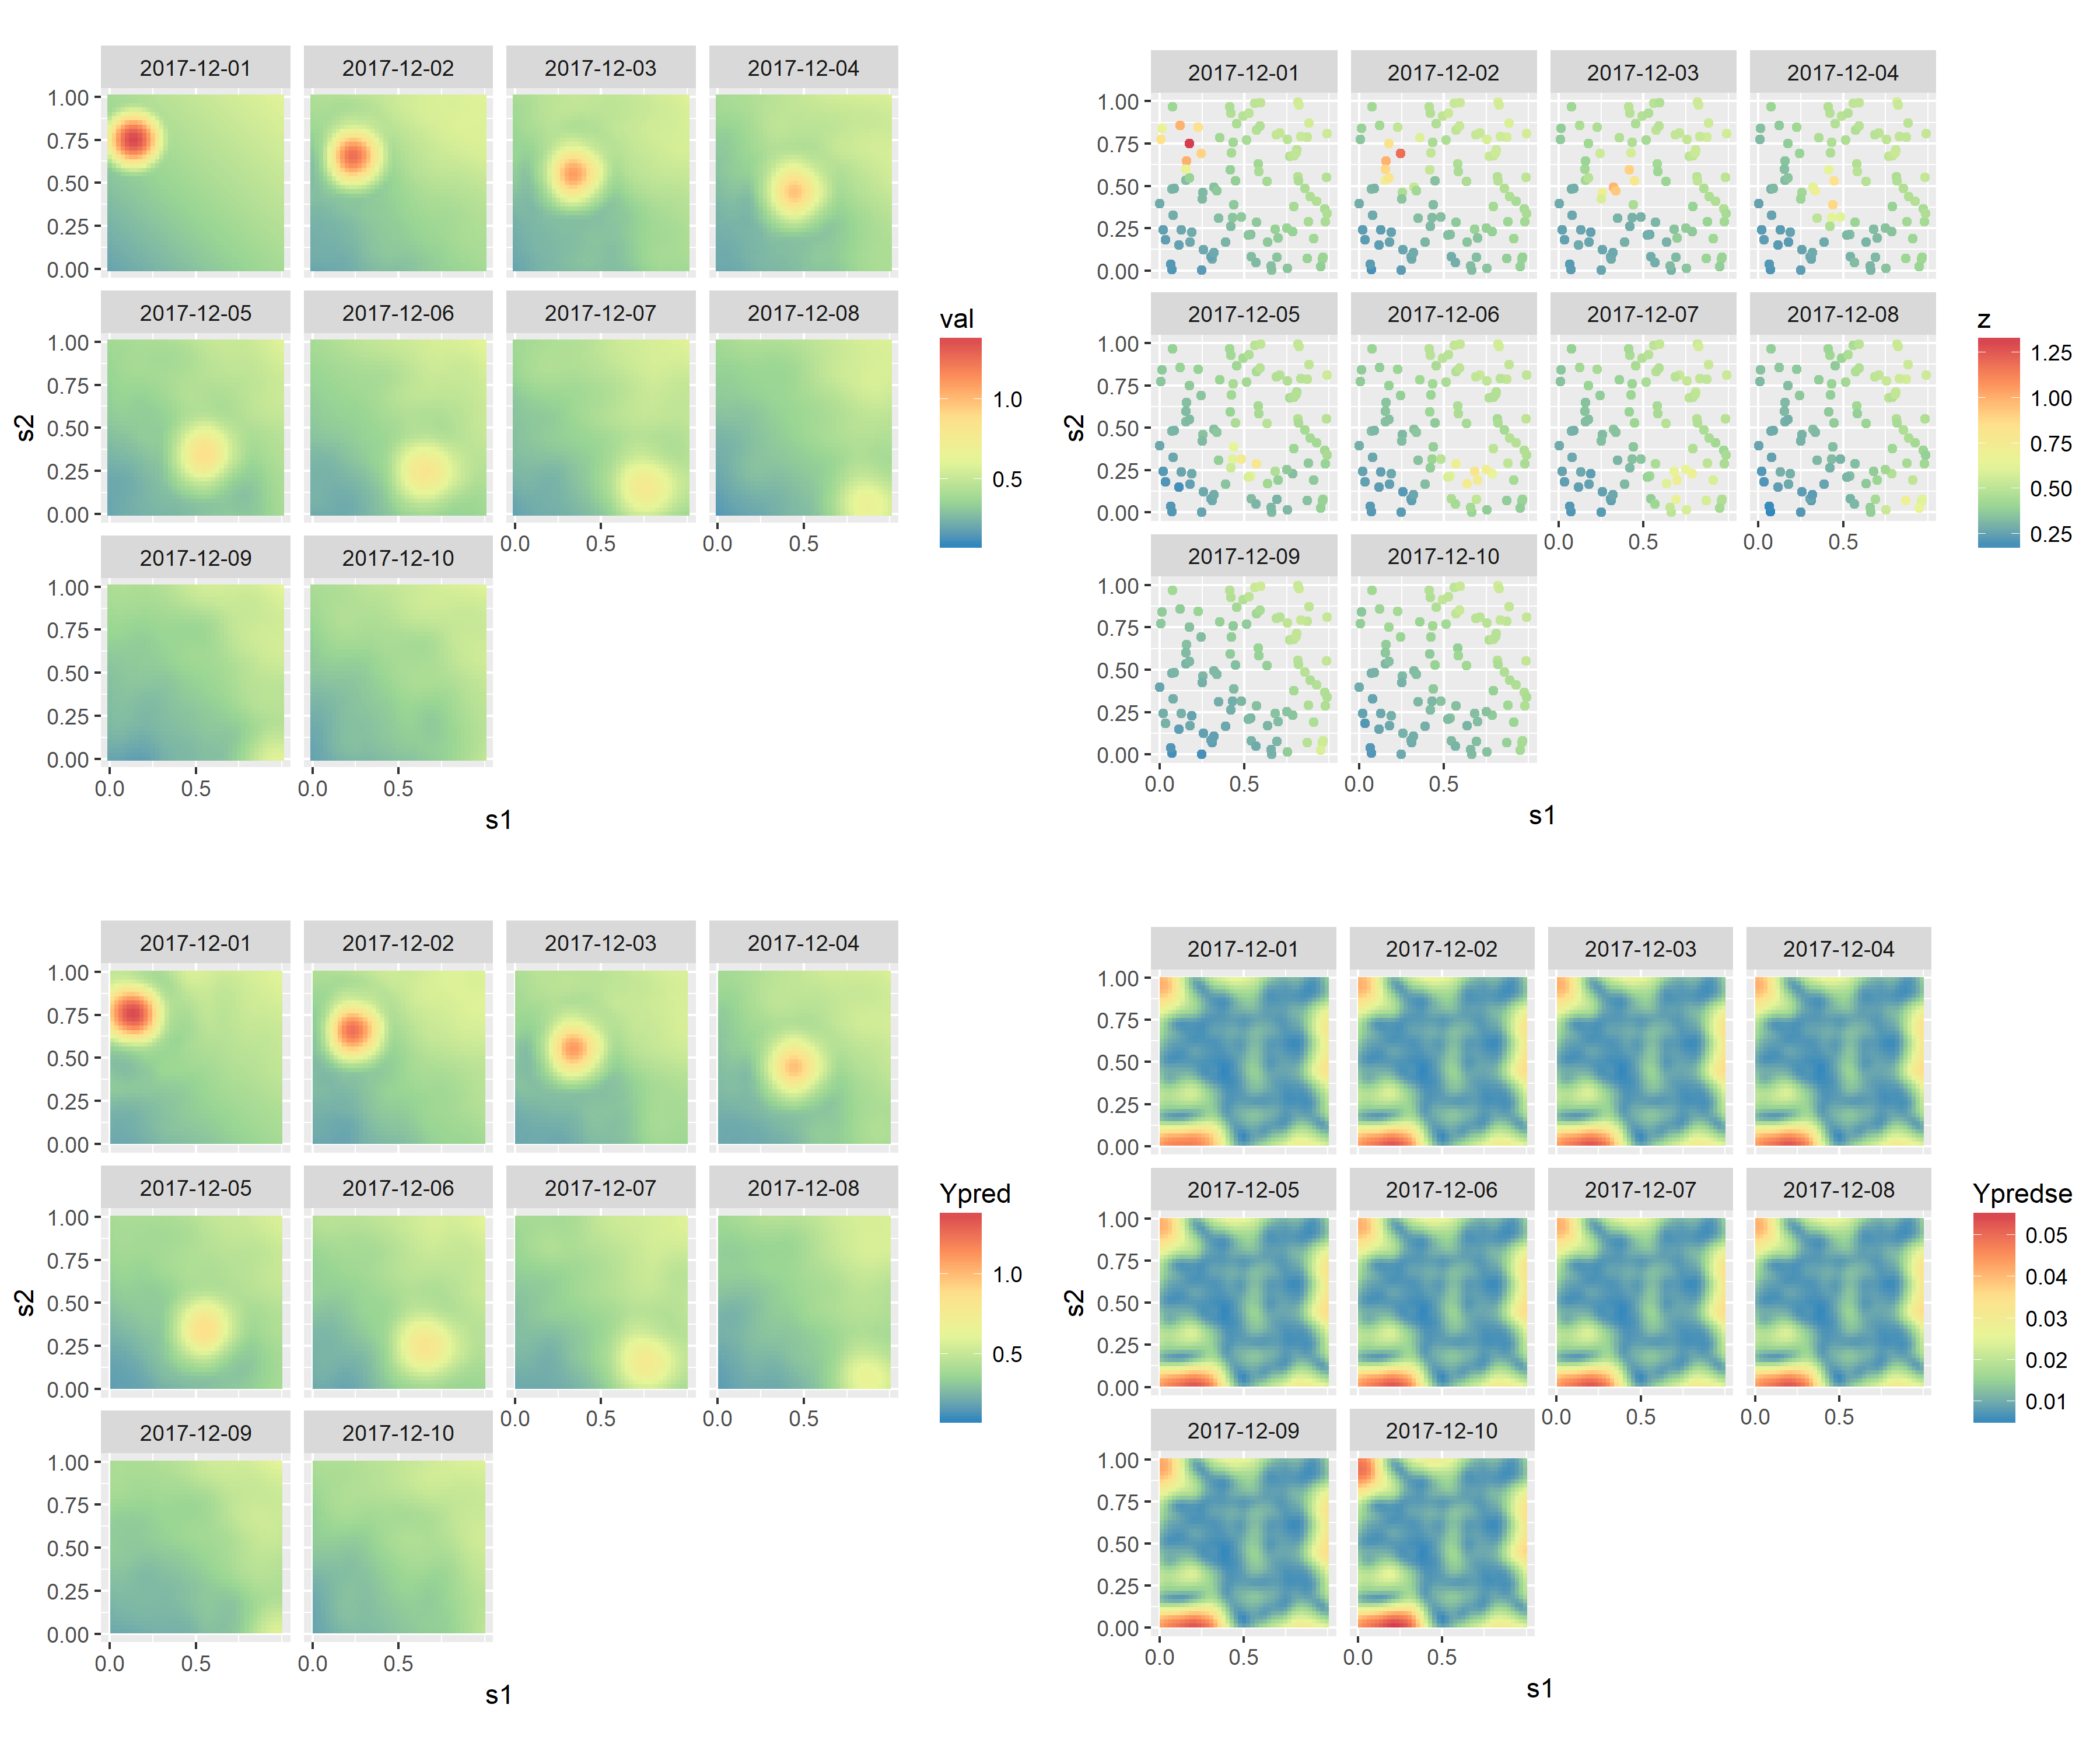
\includegraphics[width=\linewidth,angle=0]{IDEsimresults.png}
\end{center}
\caption{Simulated process (top-left panel), simulated data (top-right panel), predictions following the fitting of the IDE model (bottom-left panel) and the respective prediction standard errors (bottom-right panel).}
\label{fig:IDEsimresults}
\end{figure}



\subsection*{Simulation example with a spatially-varying kernel}

In the previous example we considered the case of a spatially-invariant kernel, that is, the case when the kernel $m(\bs,\br;\bftheta_p)$ is just a function of $\|\br - \bs\|$. In this example we consider the case when one or more of the $\bftheta_p$ are allowed to be spatially-referenced. Such models are needed when the spatio-temporal process exhibits, for example, considerabe spatially-varying drift. One such process can be simulated using the function \fn{simIDE} and specifying \args{k\_spat\_invariant}\cc{ = }\num{0}. To model such data we need to have a large \args{nobs} and many time points, and we set \args{T}\cc{ = }\num{15}. This is important, as it is difficult to obtain reasonable estimates of spatially distributed parameters unless the data covers a large part of the spatial domain for at least a few consecutive time points.

\begin{knitrout}
\definecolor{shadecolor}{rgb}{0.969, 0.969, 0.969}\color{fgcolor}\begin{kframe}
\begin{alltt}
\hlstd{SIM2} \hlkwb{<-} \hlkwd{simIDE}\hlstd{(}\hlkwc{T} \hlstd{=} \hlnum{15}\hlstd{,} \hlkwc{nobs} \hlstd{=} \hlnum{1000}\hlstd{,} \hlkwc{k_spat_invariant} \hlstd{=} \hlnum{0}\hlstd{)}
\end{alltt}
\end{kframe}
\end{knitrout}

As above, the process and the data can be plotted through

\begin{knitrout}
\definecolor{shadecolor}{rgb}{0.969, 0.969, 0.969}\color{fgcolor}\begin{kframe}
\begin{alltt}
\hlkwd{print}\hlstd{(SIM2}\hlopt{$}\hlstd{g_truth)}
\hlkwd{print}\hlstd{(SIM2}\hlopt{$}\hlstd{g_obs)}
\end{alltt}
\end{kframe}
\end{knitrout}

\noindent Note how the field appears to rotate quickly anti-clockwise and arrive to a nearly complete standstill towards the lower part of the domain. The spatially-varying advection that generated this field can be visualized using

\begin{knitrout}
\definecolor{shadecolor}{rgb}{0.969, 0.969, 0.969}\color{fgcolor}\begin{kframe}
\begin{alltt}
\hlkwd{show_kernel}\hlstd{(SIM2}\hlopt{$}\hlstd{IDEmodel,} \hlkwc{scale} \hlstd{=} \hlnum{0.2}\hlstd{)}
\end{alltt}
\end{kframe}
\end{knitrout}

\noindent In this command, the argument \args{scale} scales the arrow sizes by 0.2, that is, the shift per time point is five times the displacement indicated by the arrow.

Spatially-varying kernels can be introduced by specifying the argument \args{kernel\_basis} inside the call to {\bf IDE}. The basis functions that {\bf IDE} uses are the of the same class as those used by {\bf FRK}. Below we construct 9 bisquare basis functions that are equally spaced in the domain.

\begin{knitrout}
\definecolor{shadecolor}{rgb}{0.969, 0.969, 0.969}\color{fgcolor}\begin{kframe}
\begin{alltt}
\hlstd{mbasis_1} \hlkwb{<-} \hlkwd{auto_basis}\hlstd{(}\hlkwc{manifold} \hlstd{=} \hlkwd{plane}\hlstd{(),}   \hlcom{# functions on the plane}
                       \hlkwc{data} \hlstd{= SIM2}\hlopt{$}\hlstd{z_STIDF,}  \hlcom{# data}
                       \hlkwc{nres} \hlstd{=} \hlnum{1}\hlstd{,}             \hlcom{# 1 resolution}
                       \hlkwc{type} \hlstd{=} \hlstr{'bisquare'}\hlstd{)}    \hlcom{# type of functions}
\end{alltt}
\end{kframe}
\end{knitrout}

\noindent Type \fn{show\_basis}\cc{(mbasis\_1)} to plot these basis functions.

Now, recall that $\theta_{p,1}$ corresponds to the amplitude of the kernel, $\theta_{p,2}$ to the scale or aperture, $\theta_{p,3}$ to the $x$-direction shift ``drift,'' and $\theta_{p,4}$ to the $y$-direction shift (drift). Here we decide to let $\theta_{p,1}$ and $\theta_{p,2}$ be spatially invariant (usually a reasonable assumption), and decompose $\theta_{p,3}$ and $\theta_{p,4}$ as sums of basis functions given in \cc{mbasis\_1}.

\begin{knitrout}
\definecolor{shadecolor}{rgb}{0.969, 0.969, 0.969}\color{fgcolor}\begin{kframe}
\begin{alltt}
\hlstd{kernel_basis} \hlkwb{<-} \hlkwd{list}\hlstd{(}\hlkwc{thetam1} \hlstd{=} \hlkwd{constant_basis}\hlstd{(),}
                     \hlkwc{thetam2} \hlstd{=} \hlkwd{constant_basis}\hlstd{(),}
                     \hlkwc{thetam3} \hlstd{= mbasis_1,}
                     \hlkwc{thetam4} \hlstd{= mbasis_1)}
\end{alltt}
\end{kframe}
\end{knitrout}

Modelling proceeds as before, except that now we specify the argument \args{kernel\_basis} when calling \fn{IDE}.

\begin{knitrout}
\definecolor{shadecolor}{rgb}{0.969, 0.969, 0.969}\color{fgcolor}\begin{kframe}
\begin{alltt}
\hlstd{IDEmodel} \hlkwb{<-} \hlkwd{IDE}\hlstd{(}\hlkwc{f} \hlstd{= z} \hlopt{~} \hlstd{s1} \hlopt{+} \hlstd{s2} \hlopt{+} \hlnum{1}\hlstd{,}
                \hlkwc{data} \hlstd{= SIM2}\hlopt{$}\hlstd{z_STIDF,}
                \hlkwc{dt} \hlstd{=} \hlkwd{as.difftime}\hlstd{(}\hlnum{1}\hlstd{,} \hlkwc{units} \hlstd{=} \hlstr{"days"}\hlstd{),}
                \hlkwc{grid_size} \hlstd{=} \hlnum{41}\hlstd{,}
                \hlkwc{kernel_basis} \hlstd{= kernel_basis)}
\end{alltt}
\end{kframe}
\end{knitrout}

\noindent Fitting also proceeds by calling the function \fn{fit.IDE}. Below we use the argument \args{itermax}\cc{ = }\num{400} to specify the maximum number of iterations for the optimization routine to use.

\begin{knitrout}
\definecolor{shadecolor}{rgb}{0.969, 0.969, 0.969}\color{fgcolor}\begin{kframe}
\begin{alltt}
\hlstd{fit_results_sim2} \hlkwb{<-} \hlkwd{fit.IDE}\hlstd{(IDEmodel,}
                           \hlkwc{parallelType} \hlstd{=} \hlnum{1}\hlstd{,}
                           \hlkwc{itermax} \hlstd{=} \hlnum{400}\hlstd{)}
\end{alltt}
\end{kframe}
\end{knitrout}

\noindent  As above, since this is computationally intensive, we provide cached results which can be loaded using

The fitted spatially-varying kernel can be visualized through
\begin{knitrout}
\definecolor{shadecolor}{rgb}{0.969, 0.969, 0.969}\color{fgcolor}\begin{kframe}
\begin{alltt}
\hlkwd{show_kernel}\hlstd{(fit_results_sim2}\hlopt{$}\hlstd{IDEmodel)}
\end{alltt}
\end{kframe}
\end{knitrout}
\noindent and the true and fitted spatially-varying drift parameters are shown side by side in Figure~\ref{fig:Sim2kernels}. Note how the fitted drifts capture the broad directions and magnitudes of the true model. Predictions and prediction standard errors can be obtained and visualized using \fn{predict} as above. This is left as an exercise for the reader.

\begin{figure}[t!]
\begin{center}
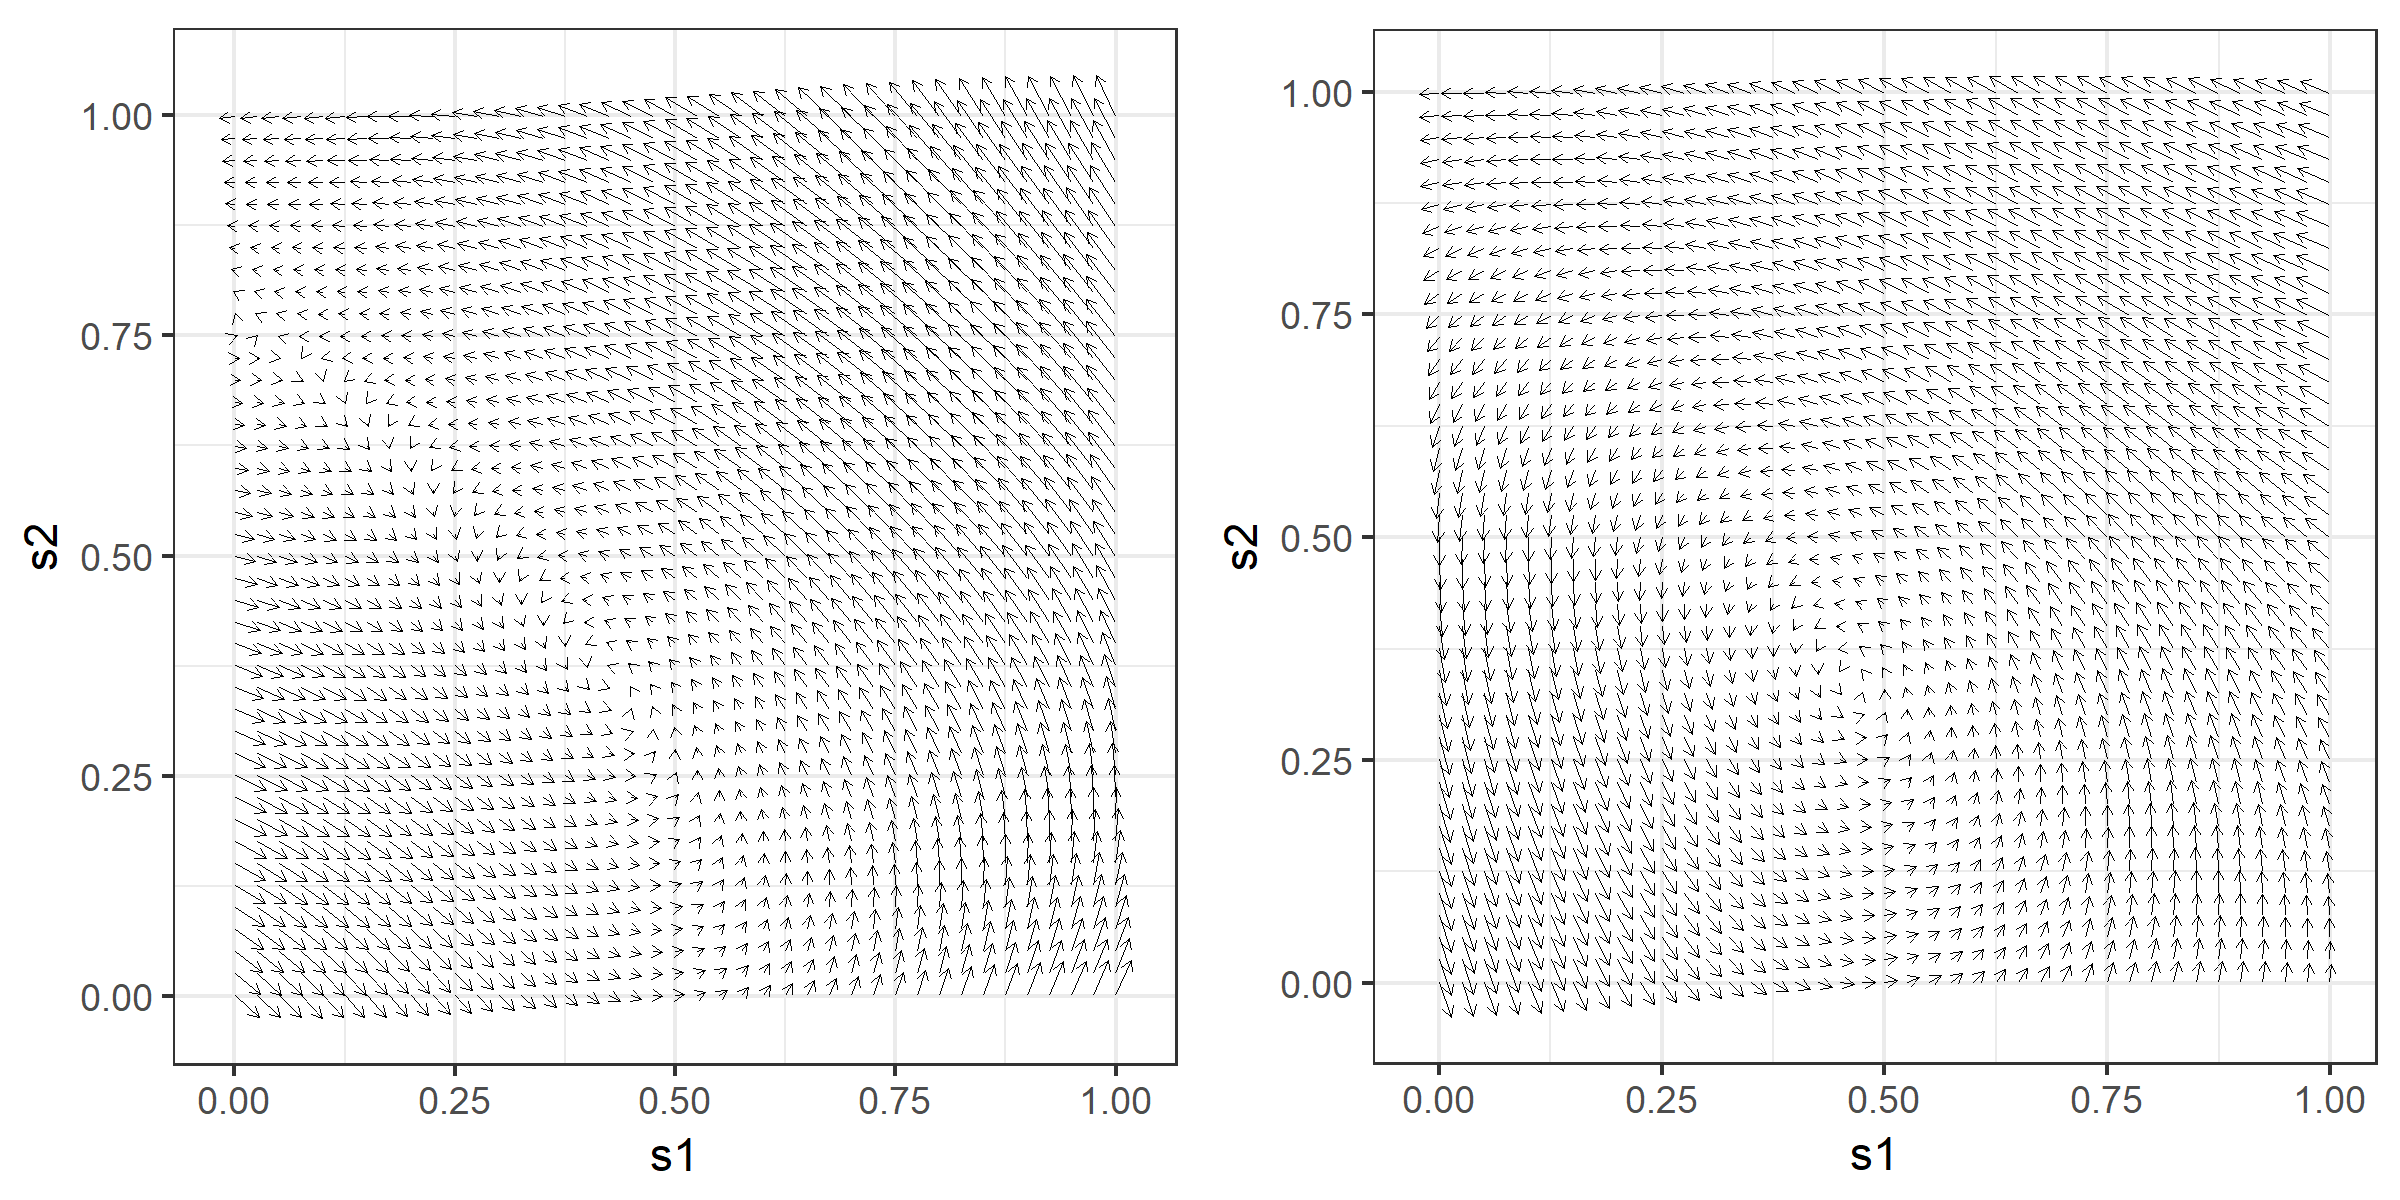
\includegraphics[width=\linewidth,angle=0]{kernels_sim2.png}
\end{center}
\caption{True drifts (left panel) and estimated drifts (right panel). \label{fig:Sim2kernels}}
\end{figure}



\end{document}
